This manual describes the procedure for building and analyzing
spatio-temporal state-space models of neural processes. Please refer
to \citet{Janoos2011}. A flowchart depiction of the algorithm
developed in that paper is shown in \Fig{fig:pipeline}

\begin{figure}[h!]
\centering {
  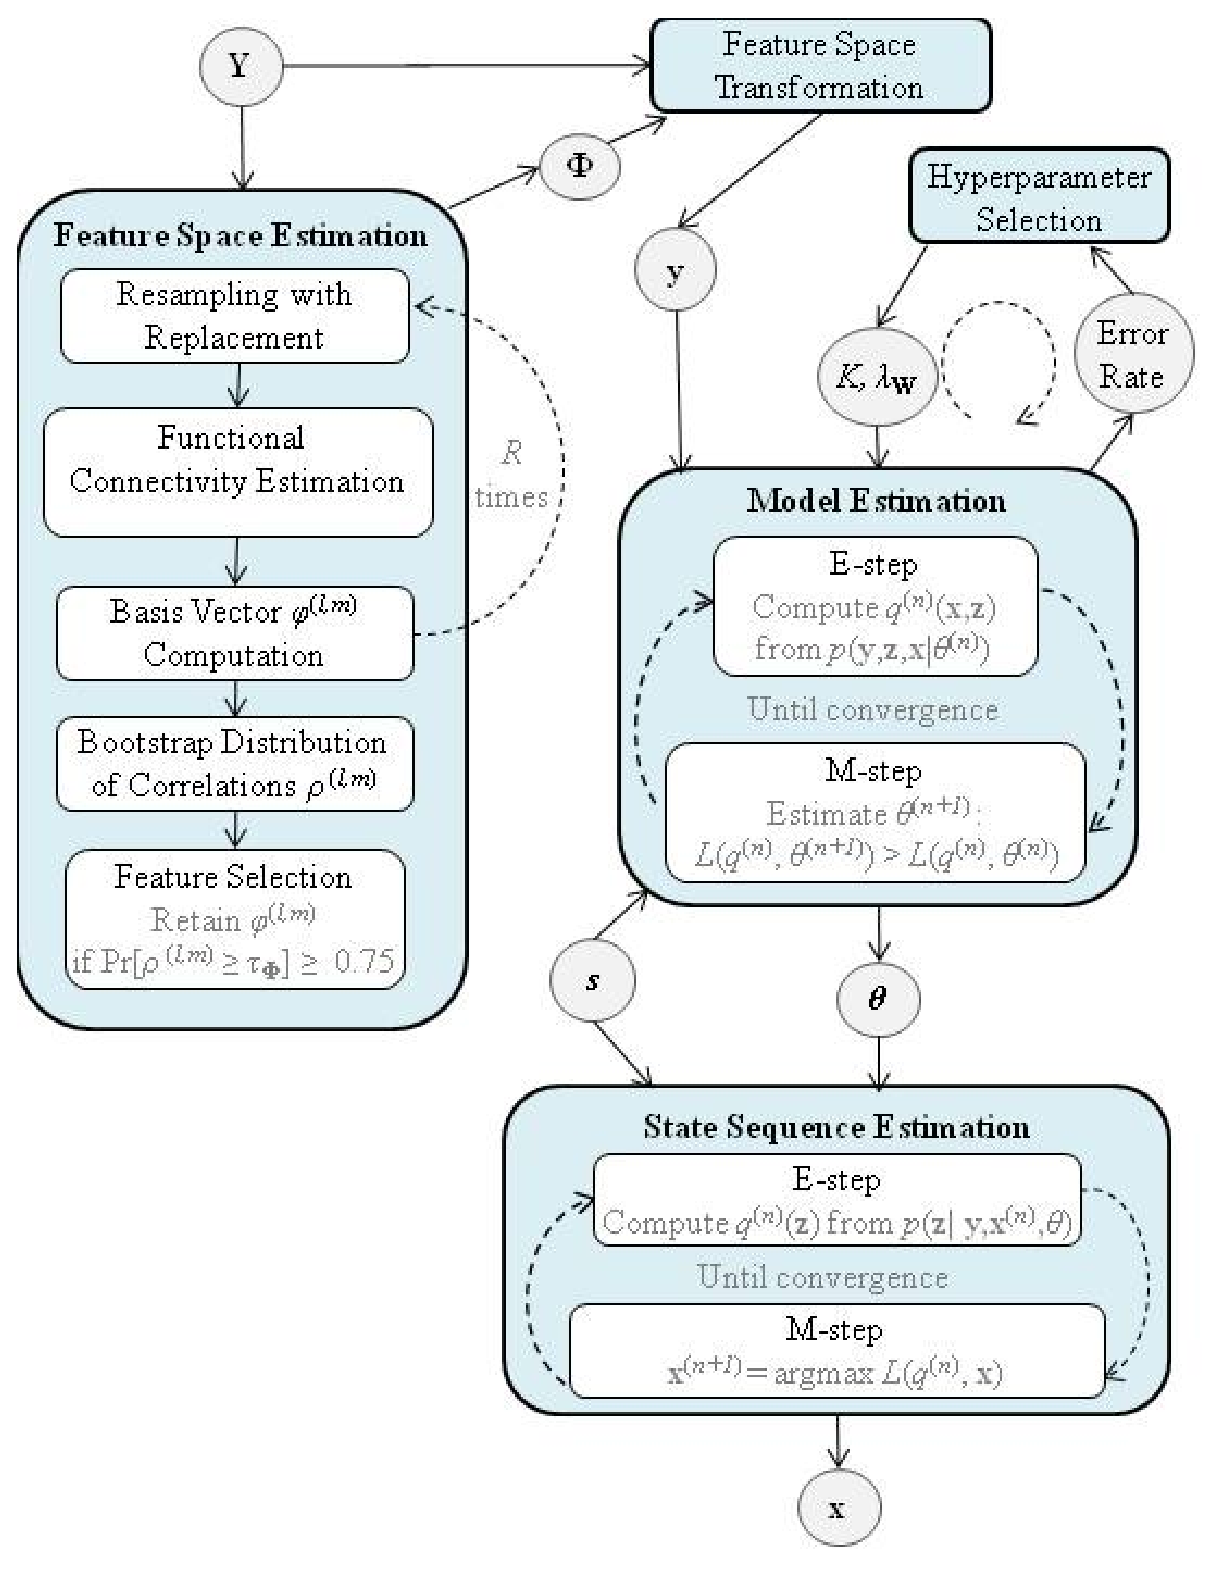
\includegraphics[width=0.8\linewidth]{pipeline-v2}}
  \caption[Outline of Method]{
  Basis vectors of the feature--space $\Phi$ are computed from the functional
  connectivity of the brain estimated from
  the fMRI data $\y$.  Dimensionality reduction is performed
  by retaining stable basis vectors using bootstrapping.
  The data ($\Y$), after projecting into the low dimensional feature--space
 are used to estimate model   parameters $\theta$ through a
  generalized EM algorithm.
  Model hyper--parameters $K$ and $\lambda_\w$ are selected
  to minimize the error of predicting the stimulus $\s$.
  Given a set of model parameters, the optimal
  state--sequence $\X^*$ is estimated using EM.
  }\label{fig:pipeline}
\end{figure}

This algorithm has been implemented in a combination of
MATLAB$^\circledR$ codes, MATLAB$^\circledR$ with
Star-P$^\circledR$, and \verb"C++".

\section{Single Session Analysis}
The main steps involved in analyzing a single session\footnote{That
is, to analyze one continuous fMRI time-series of one subject, one
session. It may consists of one actual run, or multiples runs
concatenated together. Essentially, one session is any fMRI
time-series that shares the same anatomy and imaging
characteristics.} data-set are:
\begin{enumerate}[i]
  \item Preprocessing for
  \begin{enumerate}
    \item Slice timing correction
    \item Head motion correction
    \item De-noising
    \item Head motion artifact removal
    \item Other signal artifact removal (e.g. scanner drift, pulsatile signal, respiratory signal)
  \end{enumerate}
  \item Building the feature space
  \item Specifying the experimental design
  \item Model estimation
  \item Model exploration
\end{enumerate}

\section{Multi-Subject Analysis}
In addition to the steps required for a single session analysis,
during the preprocessing step  data is spatially normalized into a
reference coordinate system using non-linear registration.

Group level analysis is performed by comparing the models across
subjects, in terms of state-space behavior and spatial activation
patterns.

\section{Prerequisites}

\subsection{Hardware}
A really fast computer / workstation to examine and explore the
results. Access to a kick-ass cluster to do the heavy duty
computation.

\subsection{Software}
\begin{enumerate}
  \item MATLAB$^\circledR$ on the work-station for design
  specification and results exploration.
  \item MATLAB$^\circledR$ with Star-P$^\circledR$ installed and
  configured, for feature-space computation and model estimation.
  \item SPM~\cite{TheFILMethodsGroup2011} version 5 or higher
  \item Group ICA of fMRI Toolbox (GIFT) \footnote{\url{http://icatb.sourceforge.net/gift}} version 1.2 or higher.
  \item An ISO Standard compatible C++ compiler.
  \item ITK\cite{Ibanez2003} version 2 or higher, installed and configured.
\end{enumerate}
